\chapter{Rôle du préfixe cyclique dans le signal OFDM}

\section{Principe du préfixe cyclique}

Avant de répondre à cette question, nous détaillerons ici le principe d'un
préfixe cyclique et nous expliciterons sa construction. Il est à noter dans un
premier temps qu'un préfixe cyclique est un intervalle de garde
particulier. ~\\

\definition{Intervalle de garde}{Un intervalle de garde est un signal de durée
  $\Delta$ que l'on place avant chaque symboles que nous souhaitons transmettre.
  Deux types d'intervalles de garde sont couramment utilisés : le préfixe
  cyclique et le bourrage de zéros.}

Le préfixe cyclique (souvent appelé CP) se place donc avant le symbole que l'on
souhaite transmettre. De plus le préfixe cyclique se construit comme la
répétition des derniers échantillons du bloc mise au début. C'est-à-dire que si
nous souhaitons transmettre $N$ états alors nous copierons $N_g$ état finaux du
symbole au début. La figure \ref{fig:PC} illustre cette copie.

\begin{figure}[!h]
  \centering
  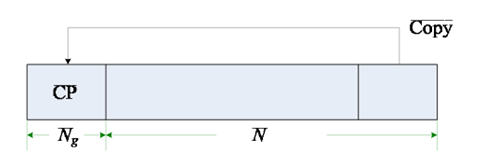
\includegraphics[width=0.7\textwidth]{pc}
  \caption{Préfixe cyclique ~\ref{supelec}} %% TODO mettre la référence
  \label{fig:PC}
\end{figure}

Pour un signal OFDM, cette copie est réalisée au niveau temporelle sous chaque
sous-porteuses.

\section{Rôle du préfixe cyclique}

\subsection{Interférence inter-symboles (ISI)}
\label{sec:ISI}

\definition{Interférence inter-symboles}{\og En télécommunications, une
  interférence inter-symbole est une forme de distorsion d'un signal qui a pour
  effet que le symbole transmis auparavant affecte le symbole actuellement
  reçu\fg{}\cite{def}}




Les symboles que nous envoyons subissent des échos. Les échos correspondent au
signal initialement envoyé mais atténué et retardé. Ils se superposent au signal
reçu de tel façon qu'a un instant $t$ il est possible de recevoir à la fois le symbole $Si$ par le
signal principal et le symbole $S_{i-1}$ par l'écho : c'est l'ISI.

Si on suppose connu le temps $T_{max}$ du retard maximal d'un écho (en pratique
il est possible de déterminer les propriétés du canal), et qu'on émet un
intervalle de garde pendant un temps $\Delta > T_{max}$ alors on recevra entre
$\Delta$ et $T_s+\Delta$ uniquement le symbole $S_i$ et l'intervalle de garde
qui est connue. Une illustration est présenté à la figure
\ref{fig:intervalleGarde}.
~\\

Le préfixe cyclique étant un intervalle de garde permet de se prémunir des
interférences entre symboles (ISI).

%Il n'y a donc plus d'ISI, on est capable d'extraire facilement l'information, le
%symbole $S_{i-1}$ n'interfère plus avec le symbole $S_i$. De plus,


\begin{figure}[!h]
  \centering
  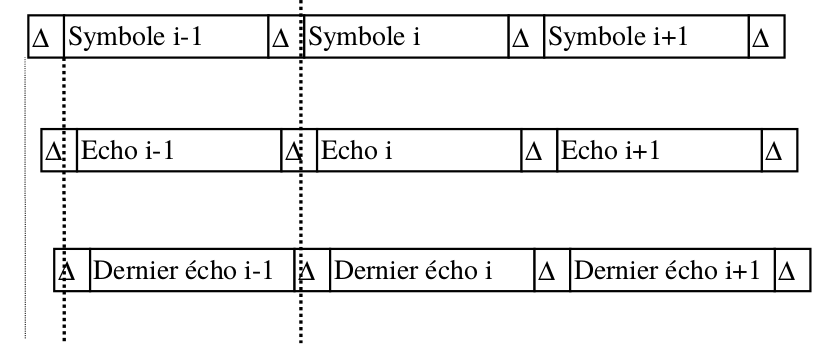
\includegraphics[width=\textwidth]{IntervalleGarde}
  \caption{Intervalle de Garde}
  \label{fig:intervalleGarde}
\end{figure}

\subsection{Interférence entre porteuses (ICI)}
\label{sec:ICI}
\definition{Interférence entre porteuses}{Interférence due au recouvrement des
  sous-porteuses en OFDM}


En OFDM, le canal est subdivisé en $N$ sous-porteuses dont les fréquences centrales
sont espacés d'un multiple de l'inverse de la période symbole $\frac{1}{T}$. De
cette manière les sous-porteuses sont orthogonales en fréquence comme on peut le
voir sur la figure \ref{fig:spectre}.

\begin{figure}[!h]
  \centering
  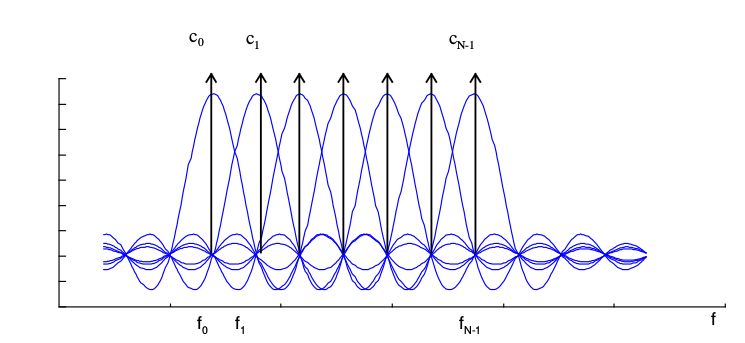
\includegraphics[width=\textwidth]{spectreOFDM}
  \caption{Spectre du signal OFDM \cite{annick}}
  \label{fig:spectre}
\end{figure}

Cette propriété est essentielle pour démoduler notre signal en réception.
Néanmoins, une légère distorsion, par exemple par effet Doppler, peut être
suffisante pour détruire cette orthogonalité et induire des recouvrements entre
les sous-porteuses. C'est ce que l'on appelle l'ICI.

Pour réduire cette interférence il faut mettre en place des techniques de
pré-égalisation et post-égalisation qui sont très coûteuses à mettre en oeuvre.
%% TODO voir si je dois citer Thomas!




Il est néanmoins possible de simplifier l'égalisation grâce au préfixe cyclique.
En effet, en introduisant de la redondance et en structurant celle-ci il est
possible de transformer le produit de convolution classique en produit de
convolution cyclique. Puis grâce à la transformée de Fourier de transformer
l'opération de convolution cyclique en produit fréquentiel scalaire. Ce calcul
est très simple à égaliser.

Dans ce cas ci c'est bien le caractère cyclique du préfixe qui permet d'éliminer
l'interférence entre porteuses (ICI).


%%% Local Variables:
%%% mode: latex
%%% TeX-master: "../rapport_de_base"
%%% End:
